\documentclass[10pt,a4paper,titlepage]{article}
\usepackage[utf8]{inputenc}

\usepackage{amsmath}
\usepackage{amsfonts}
\usepackage{amssymb}
\usepackage{graphicx}


\setlength\parindent{0pt}
\begin{document}
	
	\begin{titlepage}
		
	\title{
		\Huge Software Requirements Specification \\
		\large Software Engineering \& Project
		}
	\date{03/08/2017}
	\author{
		Team: PG-29 \\
		Phan Huy Nguyen \\
		Sean Hennessy \\
		Kin Leong Lee \\
		Pavitterjeet Sidhu \\
		Benjamin Winding \\
		Xiaoshan Chen \\
	}
	\maketitle
	
	\end{titlepage}
	
	\tableofcontents
	\newpage
	\section{Introduction}
	\subsection{Purpose}
This report is to describe the software requirements specification of the lunar rover project.

	\subsection{Document Conventions}
The document conventions in this project include the following main points....

	\subsection{Intended Audience and Reading Suggestions}
The intended audience of this document are the Client, this project team and project supervisor.

	\subsection{Project Scope}
	\paragraph{}
The scope of this project is to demonstrate a prototype for a lunar robot, which is capable of performing an automated survey of a extraterestrial landscape.
	\paragraph{}
This robot is to be constructed using the EV3 Lego Mindstorms robot provided by the client. It is to be controlled via a remote location, but is required to automatically make decisions based on the environment around it.

	\subsection{References}
1. Client Specifications, \\
2. Project Specifications, \\
3. Ev3 kit
	
	\section{Overall Description}
\subsection{Product Perspective}
The product described in this SRS is new self-contained project. It relies on the existing LEGO robot that is built by all LEGO bricks. Previously, robot cannot be controlled by human being with software no matter whether manually or automatically. This SRS defines the component of the robot system and the following diagram is identifying the functionalities and interfaces of this system.\\\\\\\\\\\\\\\\
\begin{figure}
	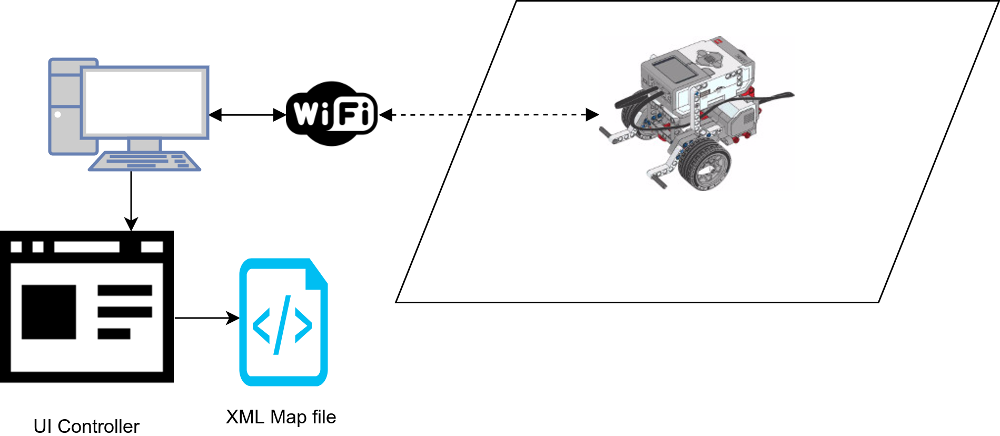
\includegraphics[width=\linewidth]{Robot_system.PNG}
	
\end{figure}

\subsection{Product Features}
The main features of this robot include
\begin{itemize}
	\item Enables the robot to map the survey area;
	\item Enables the robot to be controlled manually and automatically;
	\item Enables the robot to avoid obstacles;
	\item Enables the robot to detect the no-go zone;
	\item Enables the robot to start from the landing point and survey;
	\item Enables the robot to return the start point.
\end{itemize}

\subsection{User Classes and Characteristics}
\paragraph{}
The users of the robot include three types: students, teacher and people who only have basic knowledge of GUI control. The last type usually contains student and teacher.
\paragraph{}
Students are those who enrolled in the university of Adelaide, especially the school of computer science. There are constraints for students: they are not allowed to access the robot system, and they can only control the robot after the group members enter the password for them.
\paragraph{}
Teachers are permitted to get the password of the robot system and should not tell students the password. 
\paragraph{}
People who has basic knowledge of GUI control can also control the robot and they cannot get the password as well except for the client of this project. The client owns all privileges of this robot as long as the robot is not damaged deliberately.

\subsection{Operating Environment}
The software can be run in Window7 or above, Mac OS 10 or above, Linux and Ubuntu 16+ as long as GUI is complied using JDK (version 1.7 only). The information of hardware includes:
\begin{itemize}
	\item Window: 1 gigahertz (GHz) or faster 32-bit (x86) or 64-bit (x64) processor*;
	1 gigabyte (GB) RAM (32-bit) or 2 GB RAM (64-bit);
	16 GB available hard disk space (32-bit) or 20 GB (64-bit);
	DirectX 9 graphics device with WDDM 1.0 or higher driver.
	\item Mac: An Intel Core 2 Duo, Core i3, Core i5, Core i7, or Xeon processor;
	Mac OS X v10.6.6 or later to install via the Mac App Store (v10.6.8 recommended);
	7 GB of available disk space;
	2 GB of RAM.
\end{itemize}

\subsection{Design and Implementation Constraints}
The main constraints of design and implementation include:
\begin{itemize}
	
	\item This project is restricted using tools and the group use particular tool to do particular thing. For example, firstly, when identify the functionalities of the robot, IntelliJ is used to design and write code. Secondly, Github is used for version control and the members of group share files each other by commit. Thirdly, slack is for communication to exchange ideas or discuss some issues. Fourthly, the tool of testing functionalities of robot is ant. Also, Python is considered as writing the test script. Lastly, Latex is used for documentation since it is simple to implement professional documentation;
	\item The operating environment should meet the minimum requirements of hardware and software that mentioned in section 2.4;
	\item The version of LeJos software should be 0.9.0;
	\item The version of Java should be 7. It does not yet support version 8;
	\item Since the controller is connected with Wi-Fi and only allows the user to access, the encryption is necessary.
	\item The software only supports Lego mind storm EV3;
	\item The external code should not exceed 10 \%.
\end{itemize}
\subsection{User Documentation}
At the end of the project, a user manual would be available to users on a handbook. The handbook will mainly describe the different parts of GUI, including the getting started window, the paths and targets browser, the offline and online browser and so on, assisting users to control the robot better.

\subsection{Assumptions and Dependencies}
\paragraph{}
It is assumed that the password is entered correctly and the robot establishes connection successfully with appropriate software and hardware. Also, the robot is ready to be control manually or automatically. 	
\paragraph{}
Assumptions and dependencies include: 
\begin{itemize}
	\item Any survey area can be landing zones;
	\item The map has clear colours of track/trails;
	\item The map is flat surface;
	\item Thickness of the line is 2cm;
	\item Trail is reasonably smooth;
	\item Survey area is rectangular;
	\item Landing zone does not contain no-go zone and dangerous area.
\end{itemize}

	\section{User Requirements}
	\subsection{The Map}
    \subsubsection{The robot shall enter the survey area and produce a survey map}
    \paragraph{Description}   Upon landing, the robot shall enter the survey area and produce a survey map based on the track followed by the vehicle.
    \paragraph{Rationale}   This map will be used to analyse the survey area. This map will also be used to monitor and provide instruction to the vehicle.
    \paragraph{Acceptance criteria}   This requirement can be verified by doing a survey of an area  by using the software that we are going to develop and the survey map will be automatically produced.
    \subsubsection{The map shall be constructed in real time}
     \paragraph{Description}   After landing the robot on the predefined landing zone, the map shall be constructed in real time as long as the robot starts the survey.
    \paragraph{Rationale}   This feature will allow the remote operator to monitor and instruct the robot in real time.
    \paragraph{Acceptance criteria}   This requirement can be verified by physically observing the robot and compairing the changes on the map.
    \subsubsection{The current location of the vehicle shall be visible on map}
     \paragraph{Description}   The current location of the vehicle shall be clearly visible on the map in real time. No matter where the robot goes in the map, the operator shall be able to track the current locaton.
    \paragraph{Rationale}   This feature will allow the remote operator to track the current location of the robot. 
    \paragraph{Acceptance criteria}   This requirement can be verified by moving the robot into different directions and physically comparing the actual position of the robot between the physical map and the map on the GUI .
    \subsubsection{The map shall be able to be stored in "XML" format}
     \paragraph{Description}   The survey map which shall be created during the process of survey, shall be able to be stored in "XML" format in the system.
    \paragraph{Rationale}   This feature will allow the user to store, process, share etc the survey map.
    \paragraph{Acceptance criteria}   This requirement can be verified by storing any sample survey map in "XML" format and then veiwing it in "XML" supported plateform only. 
    \subsubsection{The software shall allow to load existing "XML" map file }
     \paragraph{Description}   The user shall be able to load any existing partial or fully completed suvey map file in "XML" format into the software. 
    \paragraph{Rationale}   This feature will allow the user to test the robot before sending it to actual survey area and will also be handy in case of system failure.
    \paragraph{Acceptance criteria}   This requirement can be verified by loading an exiting "XML" map file in the software and by allowing the robot to suvey this map.
    \subsubsection{The map shall allow to zoom in on particular area }
     \paragraph{Description}   The user shall be able to zoom in on particular area in the map by using the GUI of the software.
    \paragraph{Rationale}   This feature can be very useful if the user wants to focus on a particular area on the map and wants to have a closer and detailed look.
    \paragraph{Acceptance criteria}   This requirement can be verified by client by zooming in on a particular area of a sample map.
    \subsubsection{The map shall allow to designate NGZ any time }
     \paragraph{Description}   The remote operate shall be able to designate NGZ any time on the map by using the GUI of the software.
    \paragraph{Rationale}   This feature can be very useful in avoid any potential dangerous areas of the map detected by the remote operator.
    \paragraph{Acceptance criteria}   This requirement can be verified by drawing a few NGZ on a sample map using GUI.
	\subsection{Sensors}
    \subsubsection{The robot shall not go into craters}
     \paragraph{Description}   The robot shall detect and avoid going into carters during the survey and try to find any alternate route to destination.
    \paragraph{Rationale}   This feature will protect the robot from going into area where it is impossible for robot to recover without assistance.  
    \paragraph{Acceptance criteria}   This requirement can be verified by trying to send the robot into craters by setting the destination on other side of the carter.
    \subsubsection{ The robot shall not collide against an external object}
     \paragraph{Description}   The robot shall detect an external object and avoid colliding with it .
    \paragraph{Rationale}   This feature will protect the expensive vehicle from harm and also preserve the integrity of the survey site..
    \paragraph{Acceptance criteria}   This requirement can be verified by instructing the robot to move towards an external object.
    \subsubsection{The robot shall not go into any NGZ on map}
     \paragraph{Description}   The robot shall detect and avoid going into any NGZ available on the survey map.
    \paragraph{Rationale}   NGZ is considered as potentially dangerous area of the map in which robot shall not go. By doing so, the robot can be protected from any harm.
    \paragraph{Acceptance criteria}   This requirement can be verified by trying to send the robot into NGZ by setting the destination of the robot on other side of the NGZ.
    \subsubsection{The robot shall be able to detect a track on a given map}
     \paragraph{Description}   The robot shall be able to detect and follow any given track on the survey map.
    \paragraph{Rationale}   This will allow the operator to survey the specific area of the map.
    \paragraph{Acceptance criteria}   This requirement can be verified by loading an existing survey map with atleast one track into software and robot will detect and follow that track.
	\subsection{Operations}
    \subsubsection{The robot shall return to landing site}
     \paragraph{Description}   The robot shall remember its landing site and shall return to it when the survey is finished.
    \paragraph{Rationale}   This feature will allow the operator to bring the robot back, once the survey is finished.
    \paragraph{Acceptance criteria}   This requirement can be verified by instructing the robot to return to the landing site at any time during the survey.
    \subsubsection{The software shall provide manual control of the robot as well}
     \paragraph{Description}   The operate shall be able to take manual control of the robot at any time. 
    \paragraph{Rationale}   This feature can be useful in manually adjusting the position of the robot at any time.
    \paragraph{Acceptance criteria}   This requirement can be verified controlling the robot manully at any time using the provided GUI.
    \subsubsection{The operater shall be able to stop the robot at any time}
     \paragraph{Description}   The remote operator shall be able to stop the robot at any time using the stop button on the GUI. 
    \paragraph{Rationale}   This feature can be useful in protecting the robot or if the operator wants to abort the mission, he/she can just stop the robot and instruct it to return to the landing site.
    \paragraph{Acceptance criteria}   This requirement can be verified by pressing the stop button on GUI and in response to this, the robot will stop immediately. 
    \subsubsection{The robot shall be able to move immediately to a given point}
     \paragraph{Description}   The remote operator shall be able to place survey point on the map and the robot shall move immediately towards that point.
    \paragraph{Rationale}   This feature will allow the operator to survey any area on the map by just setting the survey point on the map.
    \paragraph{Acceptance criteria}   This feature can be verified by setting a survey point on the map using the GUI and the robot will move towards it.

	\section{System Features}
	\subsection{Map input feature}
	\subsubsection{Description and priority}
	\text This feature is designed for operator manually enter new information to the map such as NGZ, start/destination point, tracks/trails.
	\subsubsection{Stimulus/response sequence}
	\textbf{Stimulus:}
	\begin{itemize}
		\item Step 1: Open MJ Control application.
		\item Step 2: Enter username/password.
		\item Step 3: Click button “Add map info”.
		\item Step 4: Select information type from info type dropdown list (NGZ, tracks/trails etc)
		\item Step 5: Click on the map to input new map information.
		\item Step 6: Click “Save”/”Cancel” button to save or discard information input in step 5.)
	\end{itemize}
	\textbf{Response:}
	\begin{itemize}
	\item	Save new information enter by operator into map XML file.
	\end{itemize}
	\subsubsection{Functional requirements}
	\begin{itemize}
		\item \textbf{Map.InputInfo.UI} \space The application provides a UI to enter new map information.
		Map.OutputInfo.Persist: The application shall translate new map information into correct xml format and update current xml map info file with new information.
	\end{itemize}
	
	
	\subsection{Map imported/exported feature}
	\subsubsection{Description and priority}
	\text This feature designed to allow operator to import a predefine map or export current map information in xml format.
	\subsubsection{Stimulus/response sequence}
		\textbf{Stimulus:}
	\begin{itemize}
		\item Step 1: Open MJ Control application.
		\item Step 2: Enter username/password.
		\item {Step 3:}
		\begin{itemize}	
			\item \textbf{For import action:} Click “Import map” browse to existed xml map file.
			\item \textbf{For export action:} Click” Export map” system will automatically generate latest xml map information with unique name (Map-export-[current-time].xml) in “MapExport” folder of application.
		\end{itemize}
		
	\end{itemize}
	\textbf{Response:}
	\begin{itemize}
	\item Load imported map to the UI screen.
	\item Save latest info to “MapExport” folder when operator click export.
	\end{itemize}
	\subsubsection{Functional requirements}
	\begin{itemize}
		\item \textbf{Map.InputInfo.Import}: The application shall allow operator import initial map information at the beginning of the survey mission. The application shall disable import button while robot is surveying the map.
		\item \textbf{Map.OutputInfo.Export}: The application shall allow operator export map information and save it with a unique name in designated folder.
	\end{itemize}
	
	\subsection{Map display feature}
	\subsubsection{Description and priority}
	\text This feature is designed to display information of survey area in real-time and robot location. This feature also allow operator to import a xml partial map. The operators can see completed map information with zoom-in/zoom-out supported. Map will display information from imported map, manual input information from operator and real-time information return from robot while it explores the survey area (obstacle, tracks/trail, radiation areas. Etc)
	\subsubsection{Stimulus/response sequence}
	\textbf{Stimulus:}
	\begin{itemize}
	
		\item Step 1: Open MJ Control application.
		\item Step 2: Enter username/password.
		\item Step 3 (optional): Use “import map” button to browse to existing xml predefined map if there is one.
		\item Step 4 (optional): Use manual control mode or autonomous to explore survey area.
		\item Step 5 (optional): Use “Map input” feature to manual add new information to map.
		\item Step 6 (optional): Zoom-in/Zoom-out on a specific region.
		
	\end{itemize}
	\textbf{Response:}
	\begin{itemize}
		\item Realtime information displays on GUI map.
	\end{itemize}
	\subsubsection{Functional requirements}
	\begin{itemize}
		\item \textbf{Map.Import}: The application shall allow to import predefined a xml format map file which comply with predefine DTD provide by client.
		\item \textbf{Map.RealtimeDisplay}: The application shall display all information from imported map, operator inputs and survey info return from robot at real-time.
	\end{itemize}
	
	\subsection{Manual control feature }
	\subsubsection{Description and priority}
	\text This feature designated to allow operator manual control robot. It also has function to switch between manual/autonomous control and emergency stop.
	\subsubsection{Stimulus/response sequence}
	\textbf{Stimulus:}
	\begin{itemize}
		\item Step 1: Open MJ Control application.
		\item Step 2: Enter username/password.
		\item Step 3: Use navigation button on UI to control robot.
		\item Step 4: Switch between Autonomous/Manual control by turn on/off “Autonomous Control” toggle button.
		\item Step 5: Emergency stop robot by click “Emergency Stop” button
	\end{itemize}
	\textbf{Response:}
	\begin{itemize}
		\item Robot moving correct when operator use navigation buttons in manual control mode.
		\item When click on autonomous mode all navigation buttons will be disabled and robot will autonomous survey the area with internal survey algorithm.
		\item Emergency stop will stop robot intermediately both on manual/autonomous mode.
	\end{itemize}
	\subsubsection{Functional requirements}
	\begin{itemize}
		\item \textbf{Control.Manual.Navigation}: The application shall allow operator manual control robot precisely with navigation buttons.
		\item \textbf{Control.EmergencyStop}: Emergency stop button shall stop robot immediately.
		\item \textbf{Control.SwitchMode}: The application shall allow switch between manual/autonomous mode.
		\item \textbf{Map.SurveyRecord}: While robot move under manual control. All map informations collected from sensor must be recorded and display on map as describe feature 4.3.
	\end{itemize}
	
	
	\subsection{Autonomous control feature }
	\subsubsection{Description and priority}
	\text Robot have ability to self-control and autonomously survey the area. Robot also can auto navigate from one point to another point on the map after get instruction from operator.
	\subsubsection{Stimulus/response sequence}
	\textbf{Stimulus:}
	\begin{itemize}
		\item Step 1: Open MJ Control application.
		\item Step 2: Enter username/password.
		\item Step 3: Step 3: Click the Autonomous Control” toggle button to turn on autonomous mode.
		\item Step 4 (optional): Click on “Move to Location” button and enter the destination coordinate (x,y). Robot will auto navigate from current location to entered destination.
	\end{itemize}
	\textbf{Response:}
	\begin{itemize}
		\item Robot will self-control and autonomously survey area then move back to landing point after mission completed. While in autonomous mode all navigation buttons will be disabled.
	\end{itemize}
	\subsubsection{Functional requirements}
	\begin{itemize}
		\item \textbf{Control.Autonomous.Navigation}: The application shall have an self-control module which can control and navigate robot automatically corresponding to information from the map and sensors data while surveying.
		\item \textbf{Control.Autonomous.ObstacleDetectAndAvoidance}: The application shall have an obstacle detection algorithms that prevent robot collide with obstacle or move into NGZs/Craters.
		\item \textbf{Control.Autonomous.PathFinding}: The application shall have a build in algorithm to find the safe and shortest path to navigate from one location to another location.
		\item \textbf{Map.SurveyRecord}: While robot move under manual control. All map informations collected from sensor must be recorded and display on map as describe feature 4.3.
	\end{itemize}
 
 
	 \subsection{Authentication feature }
	 \subsubsection{Description and priority}
	 \text This feature is designed to prevent un-authorize person access to control robot.
	 \subsubsection{Stimulus/response sequence}
	 \textbf{Stimulus:}
	 \begin{itemize}
	 	\item Step 1: Open MJ Control application.
	 	\item Step 2: Enter username/password.
	 \end{itemize}
	 \textbf{Response:}
	\begin{itemize}
		\item Grant access to MJ control UI if username/password valid. Otherwise, display un-authorization message
	\end{itemize}
	 \subsubsection{Functional requirements}
	 \begin{itemize}
	 	\item \textbf{Control.Authentication:}  Application shall provide authentication step before operator can start to control robot.
	 \end{itemize}
	
	\section{External Interface Requirements}
\subsection{User Interfaces}
Graphic User Interface will be provided to allow a user to interact with the system through graphical buttons and map scene. This user interface will be implemented by using JavaFX. There are three types of buttons and two types of display area:\\

\textbf {Control Buttons:}This type of buttons is for user to control a EV3 robot.

Forward: It will make a robot to go forward.\\
Left: It will make a robot to turn left.\\
Right: It will make a robot to turn right.\\
Backward: It will make a robot to go backward.\\

\textbf {Connection Buttons:}This type of buttons is for user to connect and disconnect to a robot, and switch navigation mode.\\
Connect to a robot: It will make a user PC to connect to robot remotely.\\
Disconnect to a robot: It will make a user PC to disconnect to robot.\\

\textbf {Navigation Buttons:}This type of buttons is for user to switch a mode for robot navigation. There are two modes for robot navigation, manual control and automatic control.\\

Switch mode: It is for switching a robot navigation mode.\\

\textbf{Map Area:}\\
Users can draw a no-go zone in the map through mouse click.\\

\textbf{Message Area:}\\
It will display handled system information and error messages.\\

level 1 Information: It is about system status.\\\\
The example of Level 1 messages:\\
-Connected: Robot, Motors, Sensors\\
-Disconnected: Robot\\
-Moving forward\\
-Moving backward\\
-Turn left\\
-Turn right\\\\

Level 2 Warning: This is non-critical message.\\\\
The example of Level 2 messages:\\
-No EV3 found\\
-No XML found\\\\

Level 3 Error: This is critical message. There are several suggesting actions for user to solve this problem\\\\
The example of Level 3 messages:\\
-Fail to connect EV3\\
-Fail to open motor port\\
-Fail to open sensor port <= System reboot is required\\
-Fail to load XML file <= Please check whether the XML file is created by correct format.\\\\

The details of the user interface design will be documented in a separate user interface specification.



\subsection{Hardware Interfaces}

There are two types of interfaces in the system. Remote hardware interface is to provide GUI for a user to send a signal to robot and control it. Robot Hardware interface is to provide an interface to receive signals from remote system and control the hardware component in the robot.\\\\

\textbf{Remote Hardware Interface:}\\

The system is a software which is designed to run in a x86 based computer system. A modern PC with running in window, MacOS or Linux operation system is required for the system. All data and signal will be sent to robot through PC keyboard and mouse.\\

\textbf{Robot Hardware Interface:}\\

All hardware components such as sensors and motors in the Robot are controlled by a controller called EV3 brick. EV3 brick is also an interface to establish connection between remote system and robot. The communication is established through WIFI. The details of specification of WIFI dongle which is inserted to the Robot will be discussed in 5.4 section.\\

\textbf{The flow of data and control interaction between software and the hardware:}\\

The product is an integrated system which is running in remote system only. The robot itself will not contain any software which is required for running the system. Therefore, all data and control interactions are through WIFI module.\\

\begin{figure}[h]
	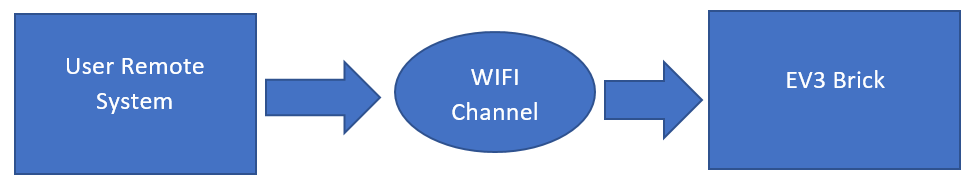
\includegraphics[width=\linewidth]{data_and_control.PNG}
	\label{fig:Flow of data and control interaction}
\end{figure}

EV3 brick will base on received signal from a user remote system to control motors and sensors.\\

\subsection{Software Interfaces}

The system is developed in Java 7 environment and support running in x-86 based computer system (Window, Linux and MacOS). The flow of software communication between each component is as below:\\\\\\\\\\\\\\\\\\\\

\begin{figure}[h]
	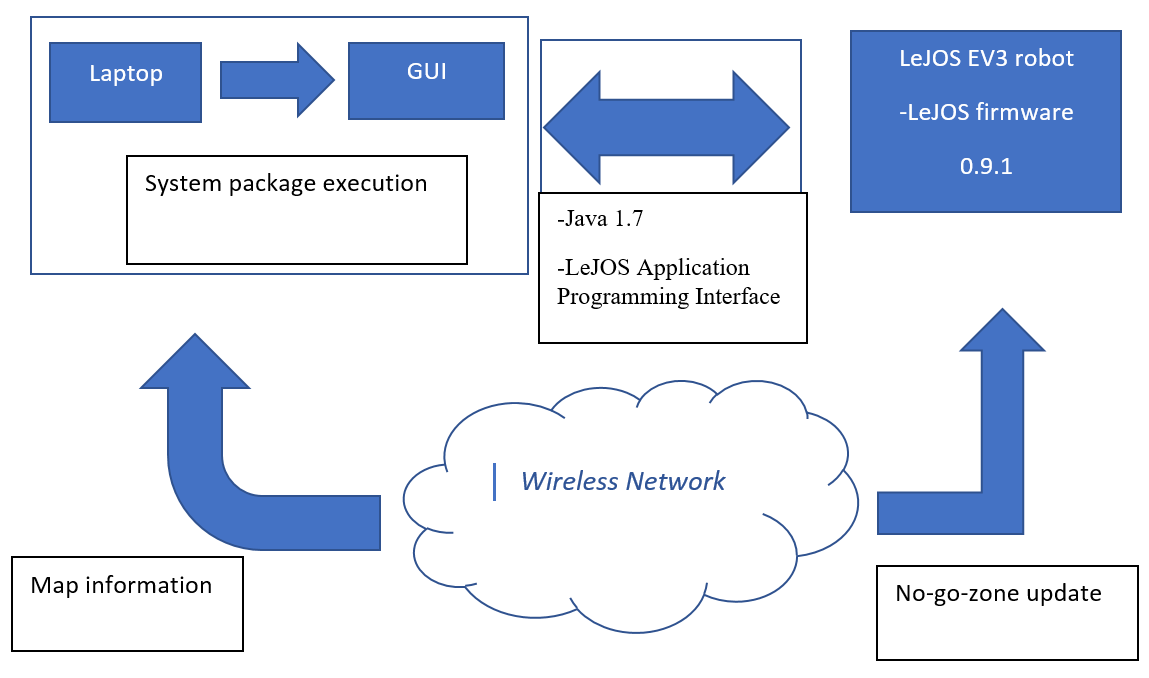
\includegraphics[width=\linewidth]{software_interface.PNG}
	\label{fig:Flow of software communication}
\end{figure}

\textbf{The details of system package:}\\

-	JDK 1.7 development environment.\\
-	LeJOS 0.9.1 library including ev3 classes.\\

These two libraries are for making a jar file which can be executed in LeJOS firmware. Also, ev3 classes provide necessary application programming interfaces for the system to communicate with robot.\\

\textbf{The detail of software components:}\\

-LeJOS EV3 is running in Linux and LeJOS EV3 0.9.1 is supporting JAVA 1.7 only.     
Therefore, the system is developed in JAVA 1.7 environment.\\

-User must execute the system via provided libraries in the system package. System package contains all necessary libraries for running the system.\\

-Robot can be controlled by user via GUI only.\\

-All data and mapping information will be transferred via wireless network. There are 100ms delay. In case of unavailable of wireless network, the system also provides Bluetooth network for communication. However, it is very unstable and longer delays is expected.\\




\textbf{LeJOS application programming interface description:}\\

Manual control:\\

Package: lejos.hardware.motor, lejos.hardware.port and lejos.hardware.sensor\\

This package of APIs is for the system to access robot’s hardware such motor and sensor.\\

Automatic control:\\

Package: lejos.robotics.navigation, lejos.robotics.pathfinding, lejos.robotics.objectdetection, lejos.robotics.mapping\\

This package of APIs is for the system to navigate the map and detect the obstacle automatically. Also, the robot will update the map information to the system.\\

The detail about mapping mechanism will provide later.\\

\subsection{Communications Interfaces}

The communication including data transfer and API communication is via wireless network (WIFI). The below is the standard for establishing wireless channel and supporting type of communication.\\

\textbf{LeJOS ev3 robot and remote system communication:}\\\\
-	The communication channel is established via WIFI.\\
-	The Digitech WIFI dongle is used for EV3 to connect wireless network (Support 802.11 b/g/n standards).\\
-	The encryption type for accessing wireless network supports WPA2 or none.\\\\
\textbf{The type of communication between LeJOS ev3 robot and remote system:}\\\\
-All system messages will be transferred to GUI display area only. It will not send any e-mail alerts to user e-mail. For the detail about what will be shown to the GUI display area, please refer to 5.1 user interface.\\
-Except for software message, the User can get the errors message about EV3 robot via SCP only since there are no external server setting in the EV3 robot.\\
-Since all functionalities are developed running remotely, all mapping information and initial map are supposed to upload to user’s PC. There are no need to transfer any document to EV3 robot.\\

	\section{Other Non-Functional Requirements}
	\subsection{Performance Requirements}
		
		\textbf {Map Accuracy}\\
		\textbf {Description:} The visual representation of the map shall be as accurate as possible. The various objects and hazards that the robot encounters must be recognized and drawn as soon as the robot encounters them.\\
		\textbf {Rationale:} The client must be able to use the map for other purposes once the crash site has been found and thereofre is relying on the map to be an accurate representation of the environment. In addition, the robot must be able to use the map to determine where past obstacles were to allow for smooth navigation and to avoid unnecessary travel time.\\

		\textbf {Speed}\\
		\textbf {Description:} The surveying of the land and discovery of the goal shall be completed in reasonable time. For this prototype, this shall be interpretted as no more than 25 minutes to complete the journey form landing to returning to the landing zone after completeing the goal. On manual control this shall be determined by the operator of the robot but will not be allowed to exceed a specified limit for safety purposes.\\
		\textbf {Rationale:} The robot will have a limited power supply and must be able to complete its mission before that power runs out. \\
		
	\subsection{Safety Requirements}
		\textbf {Significant Impact}\\
		\textbf {Description:} While on autopilot, the robot shall not exceed \begin{math}0.3 m/s\end{math}. When detecting an obstacle, the robot shall stop within 0.15 metres before collision to avoid significant impact and to allow for turning room. During prototype testing, a collison will be deemed significant impact if the robot manages to physically move an obstacle. The manual controller shall default to no more than \begin{math}0.3 m/s\end{math} however the pilot may have additional speed options available to them.\\
		\textbf {Rationale:}The safety of any persons on the landing site is paramount and a collison of the actual robot to any persons may lead to severe injury or death. The prototype is also representing a robot that will be expensive to repair and significant damage to the robot may lead to irrepairable damage and failure of the mission.\\

		\textbf{No Go Zones}\\
		\textbf {Description:} No more than half the robot may enter the NGZ at any time.\\
		\textbf{Rationale:} An NGZ may represent an area where personnel are active or may indicate an area of known hazardous materials or obstacles otherwise not detectable by the robot. For the safety of the personnel and the robot, the prototype must be able to demonstrate the ability to maneuver its way out of an NGZ without risking injury to personnel or getting stuck in an hazardous area.\\
	\subsection{Security Requirements}
		\textbf {Unauthorized Access}\\

		\textbf {Description:} The GUI shall have a login section where a username and password is presented and verified before the controller can be used.\\
		\textbf{Rationale:} Unauthorized use of the robot may lead to damage or loss if targeted by malicious competition or an individual who has not been verified by the client.\\
 
	\subsection{Software Quality Attributes}
		
		\textbf {Ease of use}\\
		\textbf {Description:} The GUI shall have intuitive controls and clearly marked buttons. The size of the contoller and map shall be set to a size that is sufficient for comfort and legibility. The visual style of the GUI will conform to the standards of similar controller layouts commonly found in maps and remote controllers.\\
		\textbf {Rationale:} The Client will have limited time to spend learning controls and must be able to intuitively navigate the GUI without much training. This should include importing and exporting map data.\\

	\section{Other Requirements}

	\section{Appendix A: Glossary}
		NGZ: No-Go Zone

	\section{Appendix B: Analysis Models}

	\section{Appendix C: Issues List}

\end{document}


